%\renewcommand{\theequation}{\theenumi}
%\begin{enumerate}[label=\thesection.\arabic*.,ref=\thesection.\theenumi]
%\numberwithin{equation}{enumi}

 Line $5x-y=5$ can be represented in vector form as,
\begin{align}
\label{eq:1.2.3_firstline}
\myvec{5&-1}\vec{x}=5
\end{align}

 Line $3x-y=3$ can be represented in vector form as,
\begin{align}
\label{eq:1.2.3_secondline}
\myvec{3&-1}\vec{x}=3
\end{align}
%
Also the equation of y axis is 
\begin{align}
\myvec{1&0}\vec{x}=0
\label{eq:1.2.3_yaxis}
\end{align}

Let line \eqref{eq:1.2.3_firstline} and  line \eqref{eq:1.2.3_secondline} meet at point $\vec{A}$.Then, 
\begin{align}
\myvec{5&-1\\3&-1}\vec{A} =\myvec{5\\3}
\\
\vec{A}={\myvec{5&-1\\3&-1}}^{-1}\myvec{5\\3}
\\
\vec{A}=\myvec{1\\0}
\end{align}

Let line \eqref{eq:1.2.3_firstline} and  line \eqref{eq:1.2.3_yaxis} meet at point $\vec{B}$. Then, 
\begin{align}
\myvec{5&-1\\1&0}\vec{B} =\myvec{5\\0}
\\
\vec{B}={\myvec{5&-1\\1&0}}^{-1}\myvec{5\\0}
\\
\vec{B}=\myvec{0\\-5}
\end{align}

Let line \eqref{eq:1.2.3_secondline} and  line \eqref{eq:1.2.3_yaxis} meet at point $\vec{C}$. Then, 
\begin{align}
\myvec{3&-1\\1&0}\vec{C} =\myvec{3\\0}
\\
\vec{C}={\myvec{3&-1\\1&0}}^{-1}\myvec{3\\0}
\\
\vec{C}=\myvec{0\\-3}
\end{align}
So, $\triangle ABC$ is formed by intersection of \eqref{eq:1.2.3_firstline},\eqref{eq:1.2.3_secondline} and \eqref{eq:1.2.3_yaxis}. The  following Python code generates Fig. \ref{fig:1.2.3_tri_py}
%
The lines \eqref{eq:1.2.3_firstline} and \eqref{eq:1.2.3_secondline} and the triangle ABC formed by the two lines and y-axis are plotted in the figure below
\begin{lstlisting}
codes/triangle/linesandtri.py
\end{lstlisting}
\begin{figure}[!ht]
\centering
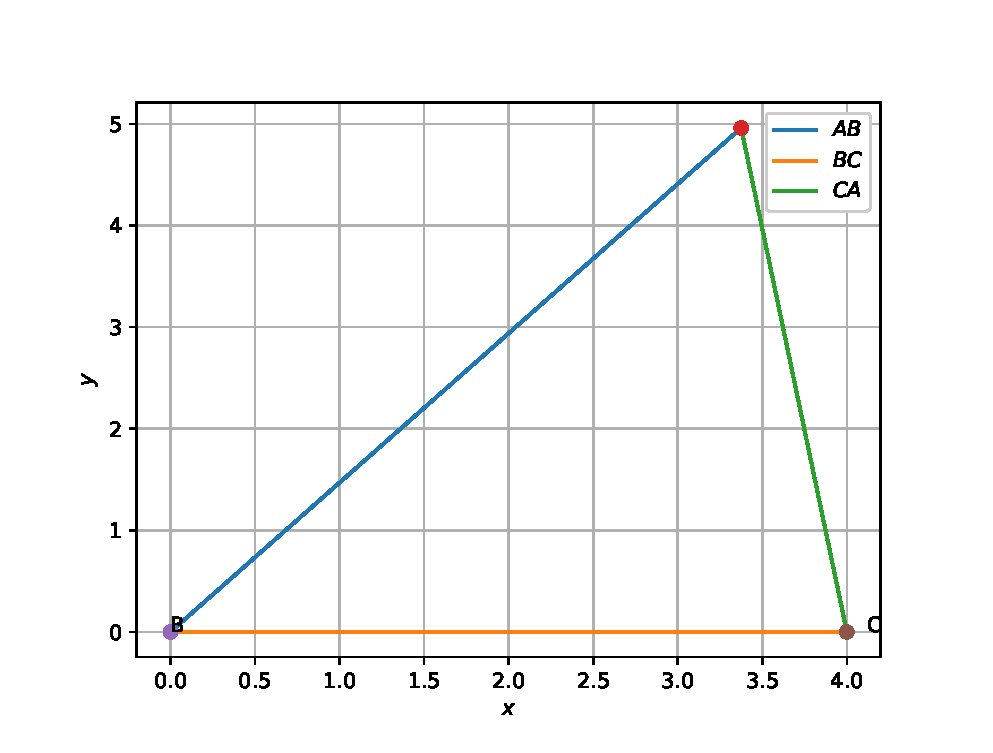
\includegraphics[width=\columnwidth]{./solutions/3/codes/triangle/pyfigs/triangle.eps}
\caption{Plot of lines and the Triangle ABC }
\label{fig:1.2.3_tri_py}
\end{figure}

%\end{enumerate}
